\subsubsection{\stid{1.07} Exascale MPI} \label{subsubsect:mpich}
\paragraph{Overview}

MPI has been the de facto standard programming model for HPC from the
mid 90's till today, a period where supercomputing performance
increased by six orders of magnitude.  The vast majority of DOE's
parallel scientific applications running on the largest HPC systems
use MPI. These application codes represent billions of dollars of
investment. Therefore, MPI must evolve to run as efficiently as
possible on Exascale systems. Our group at Argonne developed a
high-performance, production-quality MPI implementation, called MPICH.
The focus areas of the Exascale MPI / MPICH project are: (1)
continuous improvement of the performance and capabilities of the
MPICH software to meet the demands of ECP and other broader DOE
applications, (2) coordinate vendor and supercomputing center
interactions to ensure efficient solutions to applications, and (3) be
involved in the MPI forum and standardization efforts to ensure
continuity of the work beyond this project.

MPICH team is involved in the formation of the MPI Forum and have been
deeply involved in defining the MPI standard since 1992. MPICH has
helped prototype and define the majority of the features in the MPI
standard. As such, MPICH has been one of the most influential pieces of
software in accelerating the adoption of the MPI standard by the HPC
community. MPICH has been adopted by leading vendors into their own
derivative implementations. Examples include Intel (for Intel MPI), Cray
(for Cray MPI), IBM (for IBM PE MPI), Mellanox (for MLNX-MPI), Microsoft
(for MS-MPI), and Ohio State University (for MVAPICH). MPICH and its
derivatives are exclusively used in 7 of the top 10 supercomputers in
the world today. MPICH is the recipient of a number of awards including
an R\&D 100 award.

\paragraph{Key Challenges}

While we believe MPI is a viable programming model at Exascale, both
the MPI standard and MPI implementations have to address the
challenges posed by the increased scale, performance characteristics
and evolving architectural features expected in Exascale systems, as
well as the capabilities and requirements of applications targeted at
these systems. The key challenges are:

\begin{enumerate}

\item Interoperability with intranode programming models having a high
  thread count~\cite{Hybrid1, Hybrid2, FT2} (such as OpenMP,
  OpenACC and emerging asynchronous task models);

\item Scalability and performance over complex
  architectures~\cite{Perf1, Perf2, FT2, Perf4} (including high core
  counts, processor heterogeneity and heterogeneous memory);

\item Software overheads that are exacerbated by lightweight cores and
  low-latency networks;

\item Enhanced functionality (extensions to the MPI standard) based on
  experience with applications and high-level libraries/frameworks
  targeted at Exascale; and

\item Topics that become more significant as we move to the next
  generation of HPC architectures: memory usage, power, and
  resilience.

\end{enumerate}

\paragraph{Solution Strategy}

The Exascale MPI project has the following primary technical thrusts:
(1) \textbf{Performance and Scalability} (2) \textbf{Heterogeneity}
(3) \textbf{Topology Awareness} (4) \textbf{Fault Tolerance} and (5)
\textbf{MPI+X Hybrid Programming}.

Our solution strategy started by addressing performance and
scalability aspects in MPICH related to network address
management~\cite{memscal}.  Apart from this, we also looked at
communication strategies which allow the MPI library to be as
lightweight as possible~\cite{ch41, ch42}. Other solutions include
investigation and evaluation of communication relaxation hints,
investigation of optimizations to memory scalability in MPICH and
improvements to MPI RMA operations.

Exascale MPI heterogeneity efforts~\cite{Hetero1, Hetero2, Hetero3}
started with the survey on heterogeneous memory architectures on
upcoming DOE machines and how MPICH can take advantage of
them~\cite{hexe}. The efforts also included the investigation of
utilizing heterogeneous memory inside the MPI implementation and
evaluation of applications~\cite{hetero4}. The heterogeneity efforts
further extended to investigating and developing technologies for GPU
integration for the better support of the coming Exascale
supercomputers.

Exascale MPI topology awareness efforts~\cite{Topo1,Topo2} originated
with the investigation and evaluation of hints based on topology
awareness and optimizations to virtual topology functionality in
MPICH~\cite{topo-io,topo-io2}. The other efforts include investigation
of topology-aware collectives and neighborhood collectives in
MPICH~\cite{coll} and evaluation of the selected ECP applications.

Exascale MPI fault tolerance efforts~\cite{FT1, FT2} started with
support for handling noncatastrophic errors in MPI. The second effort
included defining the scope of errors in MPI, a prerequisite for
user-level failure mitigation (ULFM). Other efforts in this direction
includes standardizing ULFM in MPI and evaluating application
suitability for fault tolerance.

Exascale MPI+X hybrid programming developed firstly with effort in
improving interoperation of MPICH with threads~\cite{interthread}.
Secondly, we developed the work-queue data transfer model for
multithreaded MPI communication~\cite{workq}. We have included support
for interaction of MPICH with user-level thread (ULT)
libraries~\cite{ULT}, primarily targeting Argobots and the BOLT
runtime~\cite{BOLT}.  Other issues that are being looked at include the
investigation and evaluation on interaction between MPI and OpenMP and
the study and evaluation of MPI endpoints.

\paragraph{Recent Progress}

Figure~\ref{fig:fy19} provides the details of major milestones completed
in FY2019. In the first milestone, we studied the performance
of the RMA improvements using the large quantum chemistry application
suite NWChem (version 6.6) with ARMCI-MPI and MPICH on the Cray XC40
supercomputer. The results shown that enabling network hardware atomics
with the info hints fully eliminated the performance bottleneck in the
Density Functional Theory (DFT) module and improved the performance
scalability of NWChem DFT. In the second milestone, we studied the
performance impact of ULFM when there is no failure. A study report has
been submitted on performance analysis of the ULFM prototype. In the
third milestone, we studied the performance of MPI Endpoints. The
results shown significant improvement of using MPI endpoints
prototype---the multithreaded MPI communication reached a message rate
that is close to the case of single-threaded MPI communication. We
concluded that exposing the application level parallelism to the MPI
through the use of endpoints enables effectively scheduling of the
traffic. In such a way, multiple hardware resource can be utilized to
reduce the contention between threads and improve performance.

\begin{figure}[htb]
  \centering
  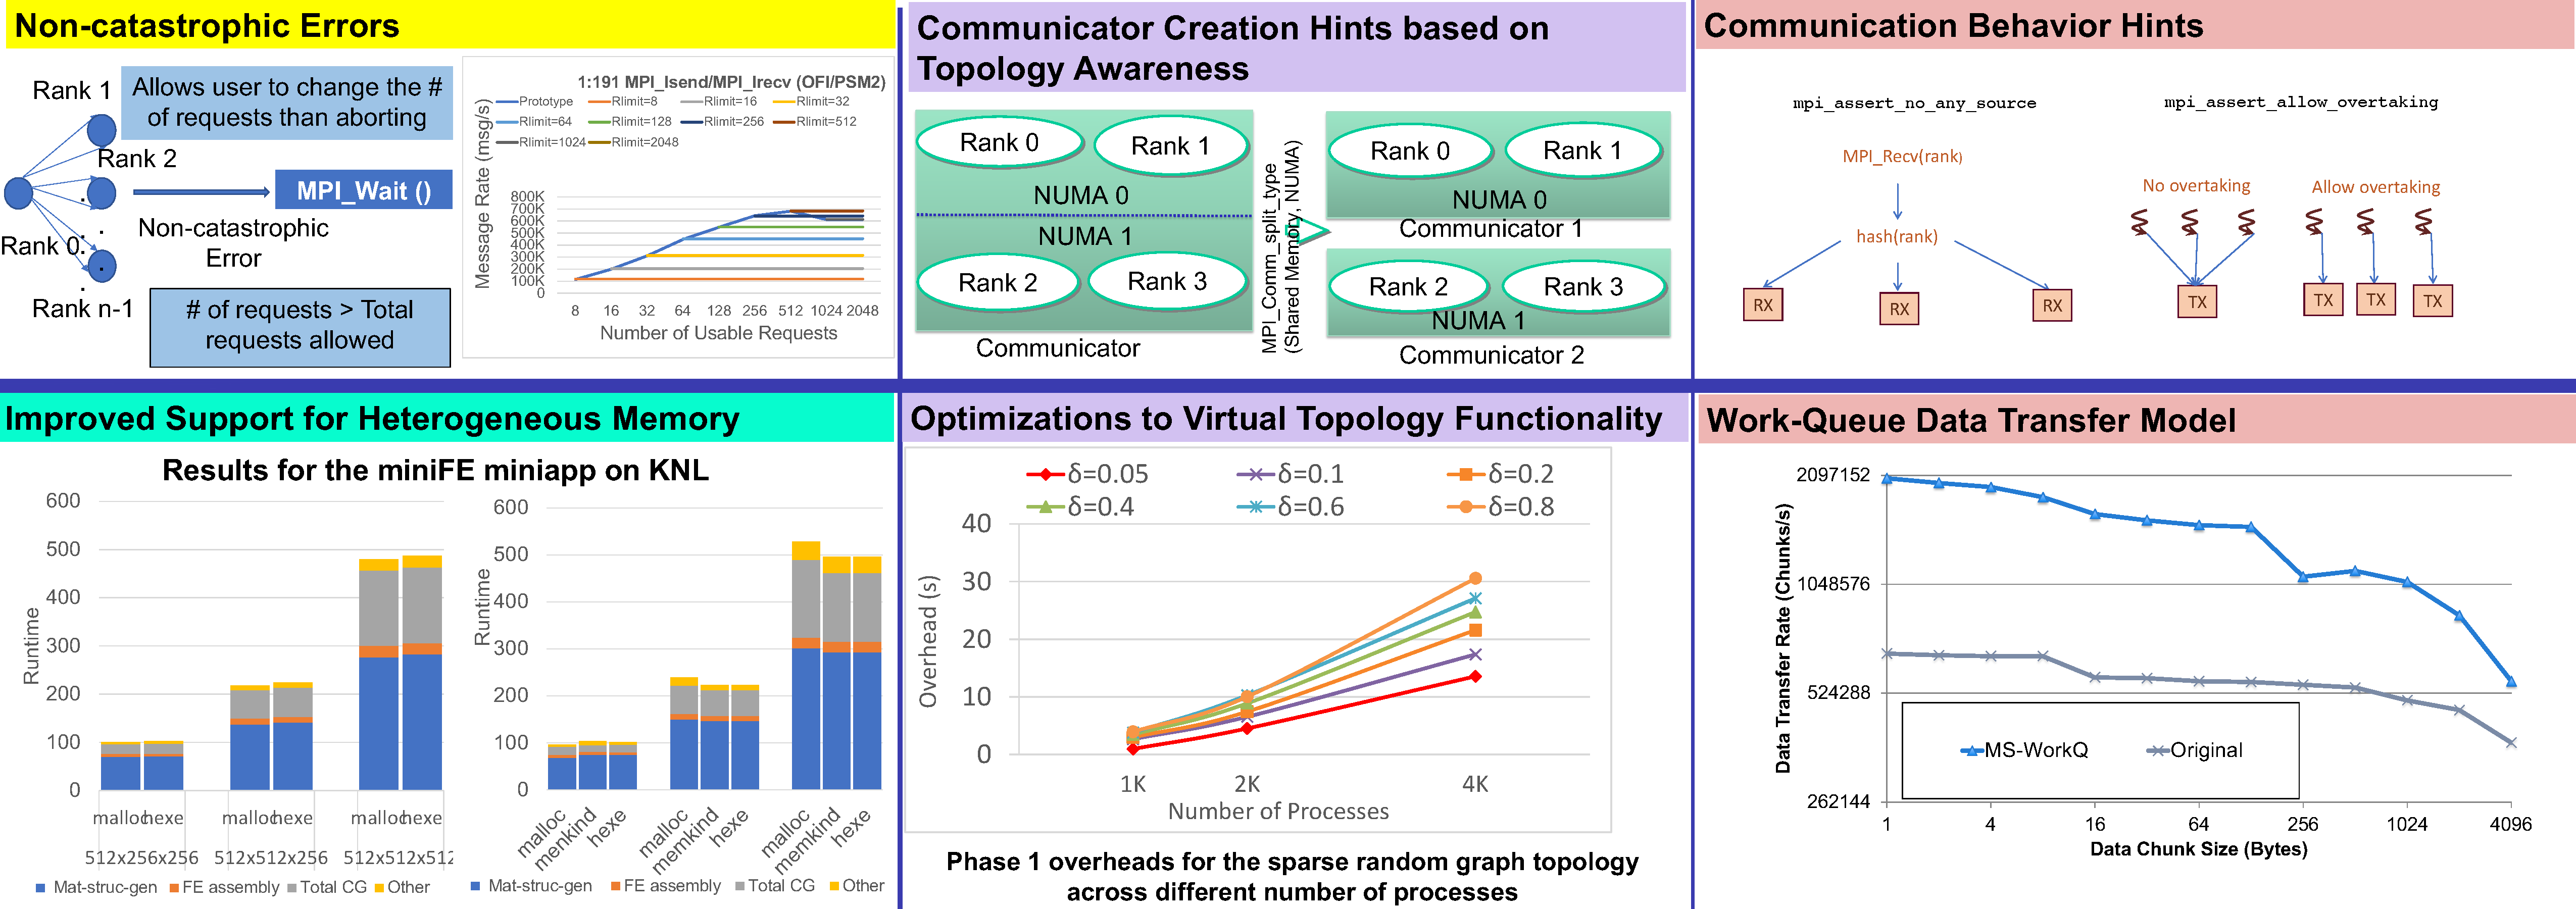
\includegraphics[width=6in]{projects/2.3.1-PMR/2.3.1.07-Exascale-MPI/MPICH-recent-milestones.pdf}
  \caption{\label{fig:fy19}Major MPICH milestones completed in fiscal year 2019}
\end{figure}

In the fourth milestone, we evaluated the benefit of using
topology-aware neighborhood collectives. We used the neighborhood
collective integration in the PETSc scalable linear solvers (KSP)
component for this evaluation. The results did show benefit, but with a
caveat that is the neighborhood collectives incurs significant setup
cost which currently overshadowing the communication benefit. The
addition of ``persistent'' collective operations in MPI-4 will allow us
to remove the per-operation setup cost. In the last milestone, we
performed comprehensive evaluation of the project which included
functional tests and performance tests.  The experiment results using
Nek5000 on OLCF Summit supercomputer shown significant improvements in
performance and scalability due to the techniques developed in this ECP
project.

\paragraph{Next Steps}
A major focus of the ongoing Exascale MPI efforts is MPI+GPU
improvements. This includes improvements for
multiple accelerator nodes and native hardware models, support for
noncontiguous data and software evaluations. Exascale MPI ongoing
efforts also includes a developing a collective selection framework for
improving the performance and scalability of collectives. We are also
making efforts in MPI standardization which includes investigation
application usage of MPI and incorporating those insights into the
MPI standard through continuous participation of the MPI standardization
process.
